\documentclass{beamer}

\usepackage[english]{babel}
\usepackage{textcmds}
\usepackage{amsthm} % for the proof-environment
\usepackage{amsmath}
\usepackage{amssymb}
\usepackage{mathtools}
\usepackage[scr=rsfs]{mathalpha}
\usepackage{subcaption}
\usepackage{sidecap}
\usepackage{wrapfig}
\usepackage{csquotes}
\usepackage[backend=biber,style=numeric]{biblatex}
\addbibresource{references.bib}
\renewcommand*{\bibfont}{\normalfont\small}
\usepackage{hyperref} %clickable table of contents
\hypersetup{
    colorlinks=false, %set true if you want colored links
    linktoc=all,     %set to all if you want both sections and subsections linked
    linkcolor=blue,  %choose some color if you want links to stand out
}
\usepackage{tikz}
\usetikzlibrary{positioning, quotes}

\title{Sructure Recognition with Graph Neural Networks}
\subtitle{A project for the lab-course \\Advanced Projects in Computational Physics 2 }
\date{February 05, 2025}
\author{Benedikt Wenzel}

\usetheme{test}
\usefonttheme[onlymath]{serif}

\begin{document}

\begin{frame}[plain]
\hspace*{-0.7cm}
\begin{minipage}{\textwidth}
    \titlepage    
\end{minipage}
\end{frame}

\begin{frame}
    \frametitle{Table of contents}
    \tableofcontents
\end{frame}

\section{Theoretical Background}
\subsection{A Few More Words on Message Passing}
\begin{frame}
    \frametitle{Theoretical Background - Message Passing}
    \textbf{Overview:}
\begin{figure}
    \centering
    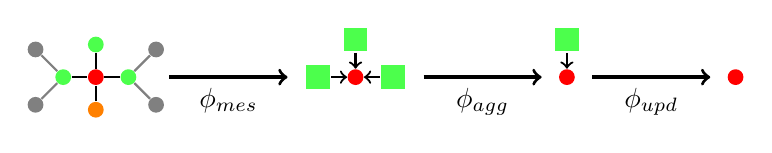
\begin{tikzpicture}[
        node distance=0.2cm and 0.2cm,
        node_g/.style={circle, inner sep=0pt, fill=green!70, minimum size=2mm}, 
        node_r/.style={circle, inner sep=0pt, fill=red, minimum size=2mm},
        node_o/.style={circle, inner sep=0pt, fill=orange, minimum size=2mm},
        node/.style={circle, inner sep=0pt, fill=gray, minimum size=2mm},
        mess/.style={rectangle, fill=green!70, very thick, minimum size=3mm},
        node_missing/.style={circle, inner sep=0pt, fill=white, minimum size=2mm}
        ]  
        %Nodes step 1
        \node[node_r] (centernode)                          {};
        \node[node_g] (top)           [above=of centernode]   {};
        \node[node_o] (bottom)        [below=of centernode]   {};
        \node[node_g] (right)         [right=of centernode]   {};
        \node[node_g] (left)          [left=of centernode]    {};
        \node[node] (llt)           [above left=of left]    {};
        \node[node] (llb)           [below left=of left]    {};
        \node[node] (rrt)           [above right=of right]    {};
        \node[node] (rrb)           [below right=of right]    {};
        %Lines step 1
        \draw[-, thick]  (top.south) -- node[anchor=west]{} (centernode.north);
        \draw[-, thick] (left.east) -- node[anchor=south]{} (centernode.west);
        \draw[-, thick] (right.west) -- node[anchor=north]{} (centernode.east);
        \draw[-, thick] (centernode.south) -- (bottom.north);
        \draw[-, thick, gray] (left.north west) -- (llt.south east);
        \draw[-, thick, gray] (left.south west) -- (llb.north east);
        \draw[-, thick, gray] (right.north east) -- (rrt.south west);
        \draw[-, thick, gray] (right.south east) -- (rrb.north west);

        \node[node_missing] (stop_1) [right=of right] {};
        \node[node_missing] (start_2) [right=1.5cm of stop_1] {};
        \draw[->, very thick, black] (stop_1) -- node[anchor=north, black]{$\phi_{mes}$} (start_2);
        
        %Nodes step 2
        \node[mess] (mess_left)          [right=0cm of start_2]    {};
        \node[node_r] (centernode_2)  [right=of mess_left]     {};
        \node[mess] (mess_top)           [above=of centernode_2]   {};
        \node[mess] (mess_right)         [right=of centernode_2]   {};
         %Lines step 2
        \draw[->, thick]  (mess_top.south) -- (centernode_2.north);
        \draw[->, thick] (mess_left.east) -- (centernode_2.west);
        \draw[->, thick] (mess_right.west) -- (centernode_2.east);

        \node[node_missing] (stop_2) [right=0cm of mess_right] {};
        \node[node_missing] (start_3) [right=1.5cm of stop_2] {};
        \draw[->, very thick, black] (stop_2) -- node[anchor=north, black]{$\phi_{agg}$} (start_3);

        %Nodes step 3
        \node[node_r] (centernode_3)  [right=0cm of start_3]     {};
        \node[mess] (mess_final)      [above=of centernode_3]   {};
        %Lines step 3
        \draw[->, thick]  (mess_final.south) -- (centernode_3.north);

        \node[node_missing] (stop_3) [right=0cm of centernode_3] {};
        \node[node_missing] (start_4) [right=1.5cm of stop_3] {};
        \draw[->, very thick, black] (stop_3) -- node[anchor=north, black]{$\phi_{upd}$} (start_4);

        %Nodes step 4
        \node[node_r] (centernode_4)  [right=0cm of start_4]     {};
    
    \end{tikzpicture}
\end{figure}
\textbf{Message passing consists of three steps:}
\begin{enumerate}
    \item Computing messages ($\phi_{mes}$)
    \item Aggregating messages ($\phi_{agg}$)
    \item Updating node values ($\phi_{upd}$)
\end{enumerate}
\vfill
\end{frame}
\begin{frame}
    \frametitle{Theoretical Background - Message Passing}
    \textbf{Step 1: Compute Messages}
\begin{figure}
    \centering
    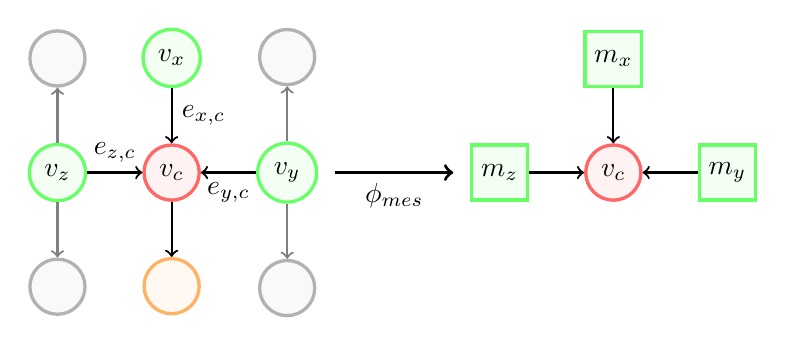
\begin{tikzpicture}[
        node distance=0.7cm and 0.7cm,
        node_r/.style={circle, draw=red!60, fill=red!5, very thick, minimum size=7mm},
        node_o/.style={circle, draw=orange!60, fill=orange!5, very thick, minimum size=7mm},
        node_g/.style={circle, draw=gray!60, fill=gray!5, very thick, minimum size=7mm},
        node/.style={circle, draw=green!60, fill=green!5, very thick, minimum size=7mm},
        mess/.style={rectangle, draw=green!60, fill=green!5, very thick, minimum size=7mm},
        node_missing/.style={circle, inner sep=0pt, fill=white, minimum size=2mm}
        ]
        %Nodes step 1
        \node[node_r] (centernode)                          {$v_c$};
        \node[node] (top)           [above=of centernode]   {$v_x$};
        \node[node_o] (bottom)        [below=of centernode]   {};
        \node[node] (right)         [right=of centernode]   {$v_y$};
        \node[node] (left)          [left=of centernode]    {$v_z$};
        \node[node_g] (llt)           [above=of left]    {};
        \node[node_g] (llb)           [below=of left]    {};
        \node[node_g] (rrt)           [above=of right]    {};
        \node[node_g] (rrb)           [below=of right]    {};
    
        %Lines step 1
        \draw[->, thick]  (top.south) -- node[anchor=west]{$e_{x,c}$} (centernode.north);
        \draw[->, thick] (left.east) -- node[anchor=south]{$e_{z,c}$} (centernode.west);
        \draw[->, thick] (right.west) -- node[anchor=north]{$e_{y,c}$} (centernode.east);
        \draw[->, thick] (centernode.south) -- (bottom.north);
        \draw[->, thick, gray] (left.north) -- (llt.south);
        \draw[->, thick, gray] (left.south) -- (llb.north);
        \draw[->, thick, gray] (right.north) -- (rrt.south);
        \draw[->, thick, gray] (right.south) -- (rrb.north);

        \node[node_missing] (stop_1) [right=0cmof right] {};
        \node[node_missing] (start_2) [right=1.5cm of stop_1] {};
        \draw[->, very thick, black] (stop_1) -- node[anchor=north, black]{$\phi_{mes}$} (start_2);

        %Nodes step 2
        \node[mess] (mess_left)          [right=0cm of start_2]    {$m_z$};
        \node[node_r] (centernode_2)  [right=of mess_left]     {$v_c$};
        \node[mess] (mess_top)           [above=of centernode_2]   {$m_x$};
        \node[mess] (mess_right)         [right=of centernode_2]   {$m_y$};
        
        %Lines step 2
        \draw[->, thick]  (mess_top.south) -- (centernode_2.north);
        \draw[->, thick] (mess_left.east) -- (centernode_2.west);
        \draw[->, thick] (mess_right.west) -- (centernode_2.east);
    \end{tikzpicture}    
\end{figure}
For $i\in\{x,y,z\}$ calculate:
\begin{equation*}
    m_i\coloneq\phi_{mes}(v_c, v_i, e_{i,c})
\end{equation*}
\end{frame}
\begin{frame}
    \frametitle{Theoretical Background - Message Passing}
    \textbf{Step 2: Aggregate Messages}
\begin{figure}
    \centering
    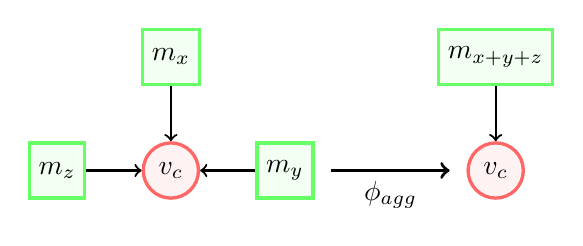
\begin{tikzpicture}[
        node distance=0.7cm and 0.7cm,
        node_r/.style={circle, draw=red!60, fill=red!5, very thick, minimum size=7mm},
        node_o/.style={circle, draw=orange!60, fill=orange!5, very thick, minimum size=7mm},
        node_g/.style={circle, draw=gray!60, fill=gray!5, very thick, minimum size=7mm},
        node/.style={circle, draw=green!60, fill=green!5, very thick, minimum size=7mm},
        mess/.style={rectangle, draw=green!60, fill=green!5, very thick, minimum size=7mm},
        node_missing/.style={circle, inner sep=0pt, fill=white, minimum size=2mm}
        ]
        %Nodes step 2
        \node[mess] (mess_left)          []    {$m_z$};
        \node[node_r] (centernode_2)  [right=of mess_left]     {$v_c$};
        \node[mess] (mess_top)           [above=of centernode_2]   {$m_x$};
        \node[mess] (mess_right)         [right=of centernode_2]   {$m_y$};
        %Lines step 2
        \draw[->, thick]  (mess_top.south) -- (centernode_2.north);
        \draw[->, thick] (mess_left.east) -- (centernode_2.west);
        \draw[->, thick] (mess_right.west) -- (centernode_2.east);

        \node[node_missing] (stop_2) [right=0cm of mess_right] {};
        \node[node_missing] (start_3) [right=1.5cm of stop_2] {};
        \draw[->, very thick, black] (stop_2) -- node[anchor=north, black]{$\phi_{agg}$} (start_3);

        %Nodes step 3
        \node[node_r] (centernode_3)  [right=0cm of start_3]     {$v_c$};
        \node[mess] (mess_final)      [above=of centernode_3]   {$m_{x+y+z}$};
        %Lines step 3
        \draw[->, thick]  (mess_final.south) -- (centernode_3.north);
    \end{tikzpicture}    
\end{figure}
Calculate total message:
\begin{equation*}
    m_{x+y+z}\coloneq\phi_{agg}(m_x,m_y,m_z)
\end{equation*}
\end{frame}
\begin{frame}
    \frametitle{Theoretical Background - Message Passing}
    \textbf{Step 3: Update node value}
\begin{figure}
    \centering
    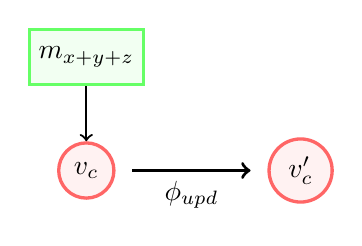
\begin{tikzpicture}[
        node distance=0.7cm and 0.7cm,
        node_r/.style={circle, draw=red!60, fill=red!5, very thick, minimum size=7mm},
        node_o/.style={circle, draw=orange!60, fill=orange!5, very thick, minimum size=7mm},
        node_g/.style={circle, draw=gray!60, fill=gray!5, very thick, minimum size=7mm},
        node/.style={circle, draw=green!60, fill=green!5, very thick, minimum size=7mm},
        mess/.style={rectangle, draw=green!60, fill=green!5, very thick, minimum size=7mm},
        node_missing/.style={circle, inner sep=0pt, fill=white, minimum size=2mm}
        ]
        %Nodes step 3
        \node[node_r] (centernode_3)  []     {$v_c$};
        \node[mess] (mess_final)      [above=of centernode_3]   {$m_{x+y+z}$};
        %Lines step 3
        \draw[->, thick]  (mess_final.south) -- (centernode_3.north);

        \node[node_missing] (stop_3) [right=0cm of centernode_3] {};
        \node[node_missing] (start_4) [right=1.5cm of stop_3] {};
        \draw[->, very thick, black] (stop_3) -- node[anchor=north, black]{$\phi_{upd}$} (start_4);

        %Nodes step 4
    \node[node_r] (centernode_4)  [right=0cm of start_4]     {$v_c'$};
    \end{tikzpicture}    
\end{figure}
Calculate new node value:
\begin{equation*}
    v_c'\coloneq\phi_{upd}(v_c, m_{x+y+z})
\end{equation*}
\textbf{Question:} What exactly are $\phi_{mes},\phi_{agg},\phi_{upd}$?
\end{frame}
\begin{frame}
    \frametitle{Theoretical Background - Message Passing}
    \textbf{Common examples for $\phi_{mes},\phi_{agg},\phi_{upd}$:}
\begin{center}
    \begin{tabular}{ c|ccc } 
        & $\phi_{mes}$ & $\phi_{agg}$ & $\phi_{upd}$\\ 
        \hline
        GCNConv (\cite{paperGCNConv}) & ? & ? \\ 
        GINEConv (\cite{paperGINEConv}) & ? & ? \\ 
    \end{tabular}
\end{center}

In general, $\phi_{mes},\phi_{agg},\phi_{upd}$ can be anything
\end{frame}

\subsection{Percolation}
\begin{frame}
    \frametitle{Theoretical Background - Percolation}
    \begin{columns}
    \begin{column}[t]{0.7\textwidth}
        Given are
        \begin{itemize}
            \item graph $G=(V,E)$
            \item one position $(n_x,n_y)$ inside unit square for each node $n\in V$
            \item small stripes at the edges of the unit square
        \end{itemize}
        $G$ is called percolating, if there are nodes $n,m\in V$ such that
        \begin{enumerate}
            \item there is a cycle containing $n$ and $m$
            \item $n$ and $m$ are connected by an edge
            \item $n$ and $m$ lie in opposite stripes
        \end{enumerate}
    \end{column} 
    \begin{column}[t]{0.3\textwidth}
        \vspace{-1cm}
        \begin{figure}[t]
            \centering
            %\hfill
            \begin{subfigure}{\textwidth}
                \centering
                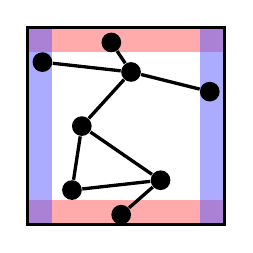
\begin{tikzpicture}[
                    node/.style={circle, inner sep=0pt, fill=black, minimum size=2.5mm}
                ]
                \useasboundingbox[fill=white](0,0) rectangle(0.625*4,0.625*4);
                \fill[red!65, fill opacity=0.5] (0,0) rectangle (0.625*4, 0.625*0.5);
                \fill[red!65, fill opacity=0.5] (0,0.625*3.5) rectangle (0.625*4, 0.625*4);
                \fill[blue!65, fill opacity=0.5] (0,0) rectangle (0.625*0.5, 0.625*4);
                \fill[blue!65, fill opacity=0.5] (0.625*3.5,0) rectangle (0.625*4, 0.625*4);
                \draw[black, very thick] (0,0) rectangle (0.625*4,0.625*4);
                \node[node] at (0.625*0.3, 0.625*3.3) (n1) {};
                \node[node] at (0.625*1.1, 0.625*2.0) (n2) {};
                \node[node] at (0.625*0.9, 0.625*0.7) (n3) {};
                \node[node] at (0.625*2.7, 0.625*0.9) (n4) {};
                \node[node] at (0.625*2.1, 0.625*3.1) (n5) {};
                \node[node] at (0.625*3.7, 0.625*2.7) (n6) {};
                \node[node] at (0.625*1.7, 0.625*3.7) (n7) {};
                \node[node] at (0.625*1.9, 0.625*0.2) (n8) {};
                \draw[very thick]  (n1) -- (n5);
                \draw[very thick]  (n5) -- (n2);
                \draw[very thick]  (n5) -- (n6);
                \draw[very thick]  (n2) -- (n4);
                \draw[very thick]  (n3) -- (n4);
                \draw[very thick]  (n2) -- (n3);
                \draw[very thick]  (n5) -- (n7);
                \draw[very thick]  (n8) -- (n4);
                \end{tikzpicture}
                \caption{non-percolating}
            \end{subfigure}
            \par\bigskip
            \begin{subfigure}{\textwidth}
                \centering
                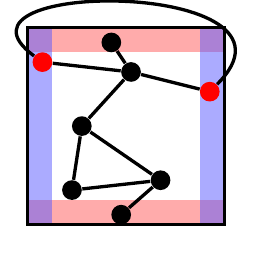
\begin{tikzpicture}[
                    node/.style={circle, inner sep=0pt, fill=black, minimum size=2.5mm},
                    node_c/.style={circle, inner sep=0pt, fill=red, minimum size=2.5mm}
                ]
                \useasboundingbox[fill=white](0,0) rectangle(0.625*4,0.625*4);
                \fill[red!65, fill opacity=0.5] (0,0) rectangle (0.625*4, 0.625*0.5);
                \fill[red!65, fill opacity=0.5] (0,0.625*3.5) rectangle (0.625*4, 0.625*4);
                \fill[blue!65, fill opacity=0.5] (0,0) rectangle (0.625*0.5, 0.625*4);
                \fill[blue!65, fill opacity=0.5] (0.625*3.5,0) rectangle (0.625*4, 0.625*4);
                \draw[black, very thick] (0,0) rectangle (0.625*4,0.625*4);
                \node[node_c] at (0.625*0.3, 0.625*3.3) (n1) {};
                \node[node] at (0.625*1.1, 0.625*2.0) (n2) {};
                \node[node] at (0.625*0.9, 0.625*0.7) (n3) {};
                \node[node] at (0.625*2.7, 0.625*0.9) (n4) {};
                \node[node] at (0.625*2.1, 0.625*3.1) (n5) {};
                \node[node_c] at (0.625*3.7, 0.625*2.7) (n6) {};
                \node[node] at (0.625*1.7, 0.625*3.7) (n7) {};
                \node[node] at (0.625*1.9, 0.625*0.2) (n8) {};
                \draw[very thick]  (n1) -- (n5);
                \draw[very thick]  (n5) -- (n2);
                \draw[very thick]  (n5) -- (n6);
                \draw[very thick]  (n2) -- (n4);
                \draw[very thick]  (n3) -- (n4);
                \draw[very thick]  (n2) -- (n3);
                \draw[very thick]  (n5) -- (n7);
                \draw[very thick]  (n8) -- (n4);
                \draw[very thick]  (n1) .. controls (-0.625*2,0.625*5) and (0.625*6,0.625*5) .. (n6);
                \end{tikzpicture}
                \caption{percolating}
            \end{subfigure}
        \end{figure}   
        \vfill     
    \end{column}   
\end{columns}
\end{frame}

\section{Goals}
\begin{frame}
    \frametitle{Goals}
    \vspace{-0.5cm}
\begin{columns}[T]
    \begin{column}{0.49\textwidth}
        \textbf{Experiment 1}\par
        \textbf{Input:} Bravais lattice (in 2D, 3D), e.g.:
        \begin{figure}
            \centering
            \includegraphics[scale=0.18]{Goals/square2d.png}                        
        \end{figure}
        \textbf{Expected output:} Bravais class, e.g. square\par
        \textbf{Question:} What are suitable choices for $\phi$'s?
    \end{column}
    \begin{column}{0.01\textwidth}
        \begin{tikzpicture}
            \draw[dashed, fauBlue, line width=\textwidth] (0,0) -- (0,7);
        \end{tikzpicture}
    \end{column}
    \begin{column}{0.49\textwidth}
        \textbf{Experiment 2}\par 
    \end{column}
\end{columns}
\end{frame}
\begin{frame}
    \frametitle{Goals}
    \vspace{-0.5cm}
\begin{columns}[T]
    \begin{column}{0.49\textwidth}
        \textbf{Experiment 1}\par
        \textbf{Input:} Bravais lattice (in 2D, 3D), e.g.:
        \begin{figure}
            \centering
            \includegraphics[scale=0.18]{Goals/square2d.png}                        
        \end{figure}
        \textbf{Expected output:} Bravais class, e.g. square\par
        \textbf{Question:} What are suitable choices for $\phi$'s?
    \end{column}
    \begin{column}{0.01\textwidth}
        \begin{tikzpicture}
            \draw[dashed, fauBlue, line width=\textwidth] (0,0) -- (0,7);
        \end{tikzpicture}
    \end{column}
    \begin{column}{0.49\textwidth}
        \textbf{Experiment 2}\par  
        \textbf{Input:} Graph inside unit-square, e.g.: 
        \begin{figure}
            \centering
            \includegraphics[scale=0.18]{Goals/nonPercolating.png}                        
        \end{figure}
        \textbf{Expected output:} percolating or not\par
        \textbf{Question:} Can this problem be solved by a GNN?
    \end{column}
\end{columns}
\end{frame}

\section{Results}
\subsection{Classification of Bravais Lattices}
\begin{frame}
    \frametitle{Results - Bravais Lattices 2D (Experiment 1)}
    which parameters have been varied, what data looks like
\end{frame}
\begin{frame}
    \frametitle{Results - Bravais Lattices 2D (Experiment 1)}
    \vspace{-.6cm}
\textbf{Averaged performance (over all 36 models):}
\begin{figure}
    \centering
    \includegraphics[width=0.7\textwidth]{Results/bravais2dAvg.png}
    \label{fig:avgBravais2d}
\end{figure}
\textbf{Question: } Do different models lead to different accuracies?

\end{frame}
\begin{frame}
    \frametitle{Results - Bravais Lattices 2D (Experiment 1)}
    \vspace*{-0.3cm}
\textbf{Best and worst performing models:}
\begin{figure}
    \centering
    \begin{subfigure}[t]{0.49\textwidth}
        \centering
        \includegraphics[width=\textwidth]{Results/bravais2dbest.png}
        \caption{Best performing model ($(d_m,w_m,d_u,w_u)=(2, 30, 1, 10)$).}
    \end{subfigure}
    \hfill
    \begin{subfigure}[t]{0.49\textwidth}
        \centering
        \includegraphics[width=\textwidth]{Results/bravais2dworst.png}
        \caption{Worst performing model ($(d_m,w_m,d_u,w_u)=(3, 30, 2, 5)$)}
    \end{subfigure}   
\end{figure}
\end{frame}
\begin{frame}
    \frametitle{Results - Bravais Lattices 2D (Experiment 1)}
    \textbf{Correlation between $w_m$ and $w_u$:}
\begin{figure}[h]
    \centering
    \includegraphics[width=0.9\textwidth]{Results/wu_vs_wm.png}
\end{figure}
\end{frame}
\begin{frame}
    \frametitle{Results - Bravais Lattices 3D (Experiment 1)}
    \vspace*{-0.3cm}
\textbf{Training of best and worst performing models on 3D dataset:}
\begin{figure}
    \centering
    \begin{subfigure}[t]{0.49\textwidth}
        \centering
        \includegraphics[width=\textwidth]{Results/bravais3dBest.png}
        \caption{Best performing model ($(d_m,w_m,d_u,w_u)=(2, 30, 1, 10)$).}
    \end{subfigure}
    \hfill
    \begin{subfigure}[t]{0.49\textwidth}
        \centering
        \includegraphics[width=\textwidth]{Results/bravais3dWorst.png}
        \caption{Worst performing model ($(d_m,w_m,d_u,w_u)=(3, 30, 2, 5)$)}
    \end{subfigure}   
\end{figure}
\end{frame}
\subsection{On the Problem of Percolation}
\begin{frame}
    \frametitle{Results - Percolation (Experiment 2)}
    why it is not possible to detect if two nodes are connected, what data looks like
\end{frame}
\begin{frame}
    \frametitle{Results - Percolation (Experiment 2)}
    \vspace{-0.5cm}
\textbf{Claim:} GNN can solve percolation problem $\implies$ GNN can solve connection problem\hfill
\newline
\begin{columns}[T]
    \begin{column}{0.7\textwidth}
        \textbf{Procedure:}
        \begin{enumerate}
            \item Start with arbitrary Graph $G$, select two nodes $n$, $m$
        \end{enumerate}        
    \end{column}    
    \begin{column}{0.3\textwidth}
        \begin{figure}
        \begin{subfigure}[]{\textwidth}
            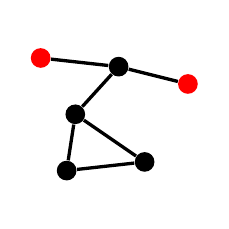
\begin{tikzpicture}[
                node/.style={circle, inner sep=0pt, fill=black, minimum size=2.5mm},
                node_c/.style={circle, inner sep=0pt, fill=red, minimum size=2.5mm}
            ]
            \useasboundingbox[fill=white](0,0) rectangle(0.55*4,0.55*4);
            \node[node_c] at (0.55*0.3, 0.55*3.3) (n1) {};
            \node[node] at (0.55*1.1, 0.55*2.0) (n2) {};
            \node[node] at (0.55*0.9, 0.55*0.7) (n3) {};
            \node[node] at (0.55*2.7, 0.55*0.9) (n4) {};
            \node[node] at (0.55*2.1, 0.55*3.1) (n5) {};
            \node[node_c] at (0.55*3.7, 0.55*2.7) (n6) {};
            \draw[very thick]  (n1) -- (n5);
            \draw[very thick]  (n5) -- (n2);
            \draw[very thick]  (n5) -- (n6);
            \draw[very thick]  (n2) -- (n4);
            \draw[very thick]  (n3) -- (n4);
            \draw[very thick]  (n2) -- (n3);
            \end{tikzpicture} 
        \end{subfigure}
        \vskip0.5cm
        \begin{subfigure}[]{\textwidth}
            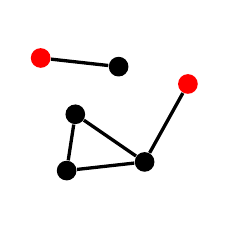
\begin{tikzpicture}[
                node/.style={circle, inner sep=0pt, fill=black, minimum size=2.5mm},
                node_c/.style={circle, inner sep=0pt, fill=red, minimum size=2.5mm}
            ]
            \useasboundingbox[fill=white](0,0) rectangle(0.55*4,0.55*4);
            \node[node_c] at (0.55*0.3, 0.55*3.3) (n1) {};
            \node[node] at (0.55*1.1, 0.55*2.0) (n2) {};
            \node[node] at (0.55*0.9, 0.55*0.7) (n3) {};
            \node[node] at (0.55*2.7, 0.55*0.9) (n4) {};
            \node[node] at (0.55*2.1, 0.55*3.1) (n5) {};
            \node[node_c] at (0.55*3.7, 0.55*2.7) (n6) {};
            \draw[very thick]  (n1) -- (n5);
            \draw[very thick]  (n2) -- (n4);
            \draw[very thick]  (n3) -- (n4);
            \draw[very thick]  (n2) -- (n3);
            \draw[very thick]  (n4) -- (n6);
            \end{tikzpicture}   
        \end{subfigure}   
        \end{figure}
    \end{column}       
\end{columns}
\end{frame}
\begin{frame}
    \frametitle{Results - Percolation (Experiment 2)}
    \vspace{-0.7cm}
\textbf{Claim:} GNN can solve percolation problem $\implies$ GNN can solve connection problem\par
\textbf{Question:} Can a GNN solve the connection problem?\par
\textbf{Answer:} No!\par
Assumption: there is a GNN with \textbf{2} layers capable of solving the connection problem\par
\begin{figure}
    \centering
    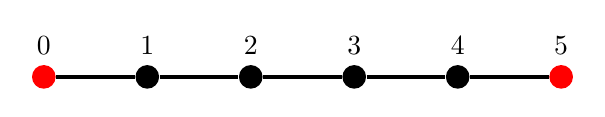
\begin{tikzpicture}[
        node/.style={circle, inner sep=0pt, fill=black, minimum size=3mm},
        node_missing/.style={circle, inner sep=0pt, fill=black, minimum size=1mm},
        node_r/.style={circle, inner sep=0pt, fill=red, minimum size=3mm}
    ]
    \node[node_r, label={$0$}] (n1) [] {};
    \node[node, label={$1$}] (n2) [right=of n1] {};
    \node[node, label={$2$}] (n3) [right=of n2] {};
    \node[node, label={$3$}] (n4) [right=of n3] {};
    \node[node, label={$4$}] (n5) [right=of n4] {};
    \node[node_r, label={$5$}] (n6) [right=of n5] {};
    \draw[very thick]  (n1) -- (n2);
    \draw[very thick]  (n2) -- (n3);
    \draw[very thick]  (n3) -- (n4);
    \draw[very thick]  (n4) -- (n5);
    \draw[very thick]  (n5) -- (n6);
    \end{tikzpicture}
\end{figure}
After one message passing steps:
\begin{figure}
    \centering
    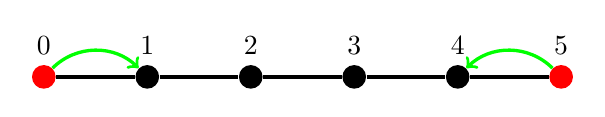
\begin{tikzpicture}[
        node/.style={circle, inner sep=0pt, fill=black, minimum size=3mm},
        node_missing/.style={circle, inner sep=0pt, fill=black, minimum size=1mm},
        node_r/.style={circle, inner sep=0pt, fill=red, minimum size=3mm}
    ]
    \node[node_r, label={$0$}] (n1) [] {};
    \node[node, label={$1$}] (n2) [right=of n1] {};
    \node[node, label={$2$}] (n3) [right=of n2] {};
    \node[node, label={$3$}] (n4) [right=of n3] {};
    \node[node, label={$4$}] (n5) [right=of n4] {};
    \node[node_r, label={$5$}] (n6) [right=of n5] {};
    \draw[very thick]  (n1) -- (n2);
    \draw[very thick]  (n2) -- (n3);
    \draw[very thick]  (n3) -- (n4);
    \draw[very thick]  (n4) -- (n5);
    \draw[very thick]  (n5) -- (n6);
    \draw [->, very thick, green] (n1) to [out=45,in=135] (n2);
    \draw [->, very thick, green] (n6) to [out=135,in=45] (n5);
    \end{tikzpicture}
\end{figure}
After two message passing step:
\begin{figure}
    \centering
    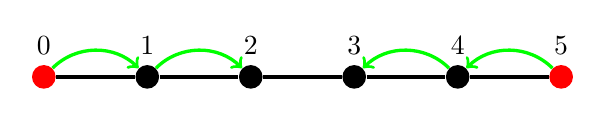
\begin{tikzpicture}[
        node/.style={circle, inner sep=0pt, fill=black, minimum size=3mm},
        node_missing/.style={circle, inner sep=0pt, fill=black, minimum size=1mm},
        node_r/.style={circle, inner sep=0pt, fill=red, minimum size=3mm}
    ]
    \node[node_r, label={$0$}] (n1) [] {};
    \node[node, label={$1$}] (n2) [right=of n1] {};
    \node[node, label={$2$}] (n3) [right=of n2] {};
    \node[node, label={$3$}] (n4) [right=of n3] {};
    \node[node, label={$4$}] (n5) [right=of n4] {};
    \node[node_r, label={$5$}] (n6) [right=of n5] {};
    \draw[very thick]  (n1) -- (n2);
    \draw[very thick]  (n2) -- (n3);
    \draw[very thick]  (n3) -- (n4);
    \draw[very thick]  (n4) -- (n5);
    \draw[very thick]  (n5) -- (n6);
    \draw [->, very thick, green] (n1) to [out=45,in=135] (n2);
    \draw [->, very thick, green] (n2) to [out=45,in=135] (n3);
    \draw [->, very thick, green] (n6) to [out=135,in=45] (n5);
    \draw [->, very thick, green] (n5) to [out=135,in=45] (n4);
    \end{tikzpicture}
\end{figure}
\end{frame}
\begin{frame}
    \frametitle{Results - Percolation (Experiment 2)}
    \vspace{-0.7cm}
\textbf{Claim:} GNN can solve percolation problem $\implies$ GNN can solve connection problem\par
\textbf{Question:} Can a GNN solve the connection problem?\par
\textbf{Answer:} No!\par
Assumption: there is a GNN with $l$ layers capable of solving the connection problem\par

\begin{figure}
    \centering
    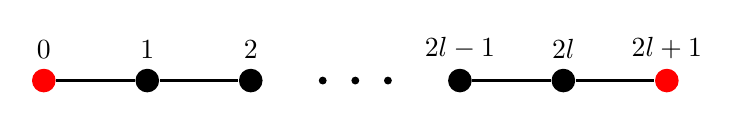
\begin{tikzpicture}[
        node/.style={circle, inner sep=0pt, fill=black, minimum size=3mm},
        node_missing/.style={circle, inner sep=0pt, fill=black, minimum size=1mm},
        node_r/.style={circle, inner sep=0pt, fill=red, minimum size=3mm}
    ]
    \node[node_r, label={$0$}] (n1) [] {};
    \node[node, label={$1$}] (n2) [right=of n1] {};
    \node[node, label={$2$}] (n3) [right=of n2] {};
    \node[node_missing] (nm_1) [right=0.7cm of n3] {};
    \node[node_missing] (nm_2) [right=0.3cm of nm_1] {};
    \node[node_missing] (nm_3) [right=0.3cm of nm_2] {};
    \node[node, label={$2l-1$}] (n4) [right=0.7cm of nm_3] {};
    \node[node, label={$2l$}] (n5) [right=of n4] {};
    \node[node_r, label={$2l+1$}] (n6) [right=of n5] {};
    
    \draw[very thick]  (n1) -- (n2);
    \draw[very thick]  (n2) -- (n3);
    \draw[very thick]  (n4) -- (n5);
    \draw[very thick]  (n5) -- (n6);
    \end{tikzpicture}
\end{figure}

\end{frame}
\begin{frame}
    \frametitle{Results - Percolation (Experiment 2)}
    \vspace{-0.5cm}
\textbf{Claim:} GNN can solve percolation problem $\implies$ GNN can solve connection problem\hfill
\newline
\begin{columns}[T]
    \begin{column}{0.7\textwidth}
        \textbf{Procedure:}
        \begin{enumerate}
            \item Start with arbitrary Graph $G$, select two nodes $n$, $m$
            \item Place $G$ inside unit square, move $n,m$ to edges, add edge ($n,m$) $\implies$ new graph $\tilde{G}$
            \item Run GNN on $\tilde{G}$
            \item $\tilde{G}$ percolating $\iff$ $n,m$ connected in $G$ 
        \end{enumerate}        
    \end{column}    
    \begin{column}{0.3\textwidth}
        \begin{figure}
        \begin{subfigure}[]{\textwidth}
            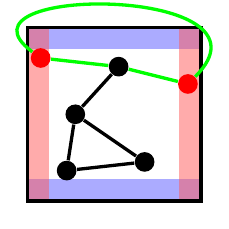
\begin{tikzpicture}[
                node/.style={circle, inner sep=0pt, fill=black, minimum size=2.5mm},
                node_c/.style={circle, inner sep=0pt, fill=red, minimum size=2.5mm}
            ]
            \useasboundingbox[fill=white](0,0) rectangle(0.55*4,0.55*4);
            \fill[blue!65, fill opacity=0.5] (0,0) rectangle (0.55*4, 0.55*0.5);
            \fill[blue!65, fill opacity=0.5] (0,0.55*3.5) rectangle (0.55*4, 0.55*4);
            \fill[red!65, fill opacity=0.5] (0,0) rectangle (0.55*0.5, 0.55*4);
            \fill[red!65, fill opacity=0.5] (0.55*3.5,0) rectangle (0.55*4, 0.55*4);
            \draw[black, very thick] (0,0) rectangle (0.55*4,0.55*4);
            \node[node_c] at (0.55*0.3, 0.55*3.3) (n1) {};
            \node[node] at (0.55*1.1, 0.55*2.0) (n2) {};
            \node[node] at (0.55*0.9, 0.55*0.7) (n3) {};
            \node[node] at (0.55*2.7, 0.55*0.9) (n4) {};
            \node[node] at (0.55*2.1, 0.55*3.1) (n5) {};
            \node[node_c] at (0.55*3.7, 0.55*2.7) (n6) {};
            \draw[very thick, green]  (n1) -- (n5);
            \draw[very thick]  (n5) -- (n2);
            \draw[very thick, green]  (n5) -- (n6);
            \draw[very thick]  (n2) -- (n4);
            \draw[very thick]  (n3) -- (n4);
            \draw[very thick]  (n2) -- (n3);
            \draw[very thick, green]  (n1) .. controls (-0.55*2,0.55*5) and (0.55*6,0.55*5) .. (n6);
            \end{tikzpicture} 
        \end{subfigure}
        \vskip0.5cm
        \begin{subfigure}[]{\textwidth}
            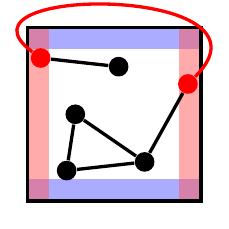
\begin{tikzpicture}[
                node/.style={circle, inner sep=0pt, fill=black, minimum size=2.5mm},
                node_c/.style={circle, inner sep=0pt, fill=red, minimum size=2.5mm}
            ]
            \useasboundingbox[fill=white](0,0) rectangle(0.55*4,0.55*4);
            \fill[blue!65, fill opacity=0.5] (0,0) rectangle (0.55*4, 0.55*0.5);
            \fill[blue!65, fill opacity=0.5] (0,0.55*3.5) rectangle (0.55*4, 0.55*4);
            \fill[red!65, fill opacity=0.5] (0,0) rectangle (0.55*0.5, 0.55*4);
            \fill[red!65, fill opacity=0.5] (0.55*3.5,0) rectangle (0.55*4, 0.55*4);
            \draw[black, very thick] (0,0) rectangle (0.55*4,0.55*4);
            \node[node_c] at (0.55*0.3, 0.55*3.3) (n1) {};
            \node[node] at (0.55*1.1, 0.55*2.0) (n2) {};
            \node[node] at (0.55*0.9, 0.55*0.7) (n3) {};
            \node[node] at (0.55*2.7, 0.55*0.9) (n4) {};
            \node[node] at (0.55*2.1, 0.55*3.1) (n5) {};
            \node[node_c] at (0.55*3.7, 0.55*2.7) (n6) {};
            \draw[very thick]  (n1) -- (n5);
            \draw[very thick]  (n2) -- (n4);
            \draw[very thick]  (n3) -- (n4);
            \draw[very thick]  (n2) -- (n3);
            \draw[very thick]  (n4) -- (n6);
            \draw[very thick, red]  (n1) .. controls (-0.55*2,0.55*5) and (0.55*6,0.55*5) .. (n6);
            \end{tikzpicture}   
        \end{subfigure}   
        \end{figure}
    \end{column}       
\end{columns}
\end{frame}
\begin{frame}
    \frametitle{Results - Percolation (Experiment 2)}
    ideas how to solve this problem
top k poooling layer explained
\end{frame}
\begin{frame}
    \frametitle{Results - Percolation (Experiment 2)}
    why we can not expect the layyer to work
results (both with and without top k)
\end{frame}

\section{Conclusion and Outlook}
\begin{frame}
    \frametitle{Conclusion and Outlook}
\end{frame}

\begin{frame}
    \frametitle{Time for Discussion and Questions}
\end{frame}
\begin{frame}
    \frametitle{References}
    \printbibliography
\end{frame}

\end{document}